\section{Resultados de Desempenho na configuração híbrida \textit{TPC-C} + \textit{CH-benCHmark}}

O objetivo desta primeira questão passa por analisar, recorrendo à configuração por defeito do PostgreSQL instalado no sistema, a \textit{performance} da execução híbrida dos \textit{benchmarks} \verb+TPC-C+ e \verb+CH-Benchmark+.

O teste consiste na execução de \textit{queries} SQL disponibilizadas pelos \textit{benchmarks}, e no qual se faz variar o \textbf{método de isolamento}, o \textbf{número de clientes} e o \textbf{número de armazéns}.

\subsection{\textit{Serializable} como Método de Isolamento}

São apresentados em seguida, sobre a forma de uma tabela, os resultados obtidos na execução do \textit{benchmark} usando como Método de Isolamento o \textit{Serializable}.

\begin{table}[!h]
\center
\small
\begin{tabular}{|c|c|c|c|c|}
\hline
\textbf{\# clientes} & \textbf{\# pedidos} & \textbf{pedidos/s} & \textbf{lat. média (s)} & \textbf{lat. perct. 99 (s)}  \\ \hline
2 & 5068 & 84.4667 & 1.0291 & 1.0702  \\ \hline
4 & 3226 & 53.7653 & 1.1079 & 2.0538  \\ \hline
8 & 1377 & 22.9500 & 1.3489 & 14.7304  \\ \hline
16 & 703 & 11.7166 & 1.8898 & 24.8298  \\ \hline
\end{tabular}
\caption{Resultados obtidos para dois (2) armazéns}
\end{table}

\begin{table}[!h]
\center
\small
\begin{tabular}{|c|c|c|c|c|}
\hline
\textbf{\# clientes} & \textbf{\# pedidos} & \textbf{pedidos/s} & \textbf{lat. média (s)} & \textbf{lat. perct. 99 (s)}  \\ \hline
2 & 2503 & 41.7166 & 1.0631 & 1.0909  \\ \hline
4 & 434 & 7.2333 & 0.9899 & 1.2105  \\ \hline
8 & 516 & 8.5999 & 2.1197 & 57.2194  \\ \hline
16 & 474 & 7.9000 & 1.6451 & 25.3641  \\ \hline
\end{tabular}
\caption{Resultados obtidos para quatro (4) armazéns}
\end{table}

\newpage

A partir dos dados exibidos nas tabelas anteriores, foram desenhados os seguintes gráficos representativos do \textbf{débito} (número de pedidos por segundo), da \textbf{latência média} e do valor do \textbf{percentil 99 da latência}, interpretada, aqui, como latência máxima.

\begin{figure}[!h]
\centering
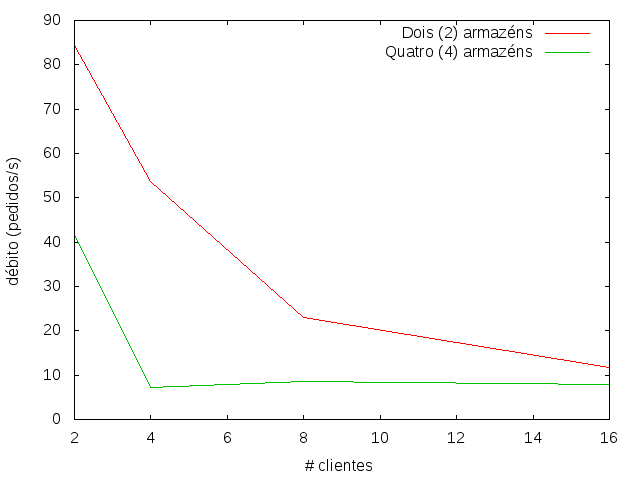
\includegraphics[scale=.4]{img/questao-1/ser-deb}
\caption{Débito obtido de acordo com o número de clientes para dois e quatro armazéns}
\end{figure}

\begin{figure}[!h]
\centering
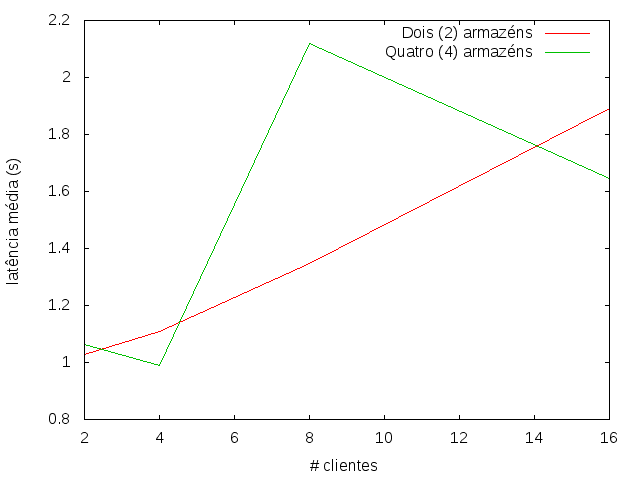
\includegraphics[scale=.4]{img/questao-1/ser-lat-med}
\caption{Latência média obtida de acordo com o número de clientes para dois e quatro armazéns}
\end{figure}

%\newpage

\begin{figure}[!h]
\centering
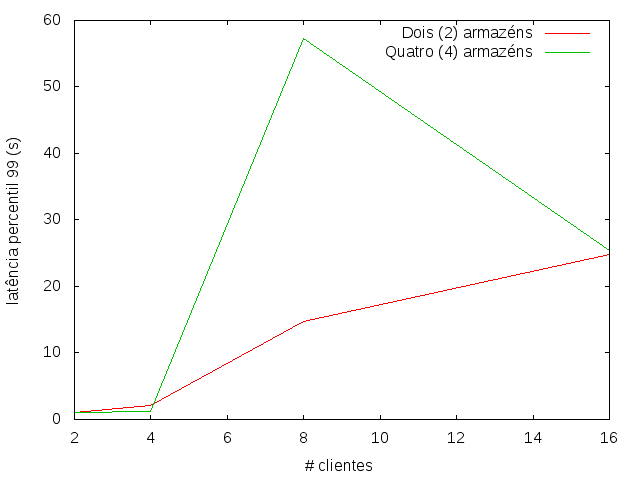
\includegraphics[scale=.4]{img/questao-1/ser-lat-pct99}
\caption{Percentil 99 da latência obtida de acordo com o número de clientes para dois e quatro armazéns}
\end{figure}

\newpage

Relativamente aos valores obtidos para o débito, observa-se uma tendêcia clara de diminuição deste à medida que o número de clientes vai aumentando, quer para dois, quer para quatro armazéns.
Verifica-se também, como seria de esperar tendo em conta o método "sequencial" de isolamento, que o débito apresenta melhores resultados para bases de dados mais com menos informação (2 armazéns).



\subsection{\textit{Repeatable Read} como Método de Isolamento}

São apresentados em seguida, sobre a forma de uma tabela, os resultados obtidos na execução do \textit{benchmark} usando como Método de Isolamento o \textit{Repeatable Read}.

\begin{table}[!h]
\center
\small
\begin{tabular}{|c|c|c|c|c|}
\hline
\textbf{\# clientes} & \textbf{\# pedidos} & \textbf{pedidos/s} & \textbf{lat. média (s)} & \textbf{lat. perct. 99 (s)}  \\ \hline
2 & 17138 & 285.6333 & 1.0078 & 1.0305  \\ \hline
4 & 18435 & 307.2458 & 1.0196 & 1.1275  \\ \hline
8 & 15426 & 257.0989 & 1.0439 & 1.2903  \\ \hline
16 & 13315 & 221.9153 & 1.0917 & 1.6116  \\ \hline
\end{tabular}
\caption{Resultados obtidos para dois (2) armazéns}
\end{table}

\begin{table}[!h]
\center
\small
\begin{tabular}{|c|c|c|c|c|}
\hline
\textbf{\# clientes} & \textbf{\# pedidos} & \textbf{pedidos/s} & \textbf{lat. média (s)} & \textbf{lat. perct. 99 (s)}  \\ \hline
2 & 16818 & 280.2991 & 1.0088 & 1.0297  \\ \hline
4 & 20372 & 339.5289 & 1.0113 & 1.1042  \\ \hline
8 & 17256 & 287.5948 & 1.0304 & 1.2829  \\ \hline
16 & 8744 & 145.7319 & 1.1217 & 2.4365  \\ \hline
\end{tabular}
\caption{Resultados obtidos para quatro (4) armazéns}
\end{table}

\newpage

A partir dos dados exibidos nas tabelas anteriores, foram desenhados os seguintes gráficos representativos do \textbf{débito} (número de pedidos por segundo), da \textbf{latência média} e do valor do \textbf{percentil 99 da latência}, interpretada, aqui, como latência máxima.

\begin{figure}[!h]
\centering
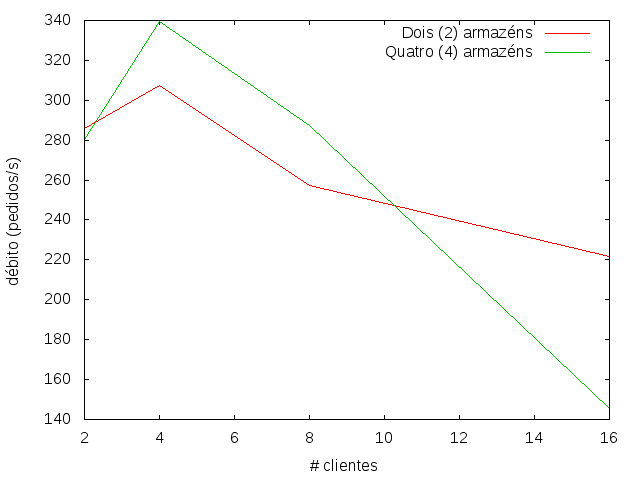
\includegraphics[scale=.4]{img/questao-1/rep-read-deb}
\caption{Débito obtido de acordo com o número de clientes para dois e quatro armazéns}
\end{figure}

\begin{figure}[!h]
\centering
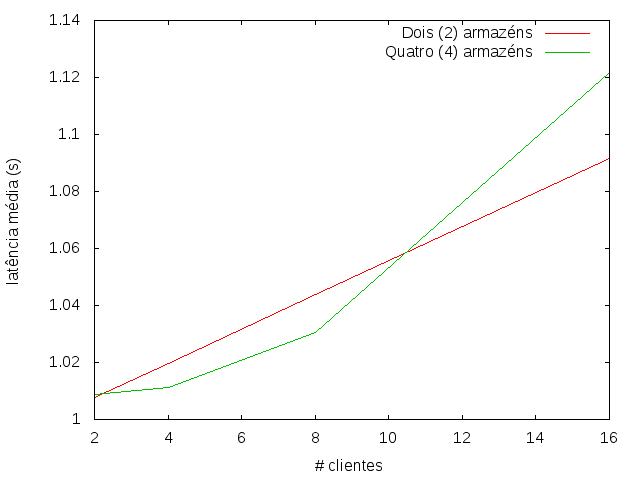
\includegraphics[scale=.4]{img/questao-1/rep-read-lat-med}
\caption{Latência média obtida de acordo com o número de clientes para dois e quatro armazéns}
\end{figure}

%\newpage

\begin{figure}[!h]
\centering
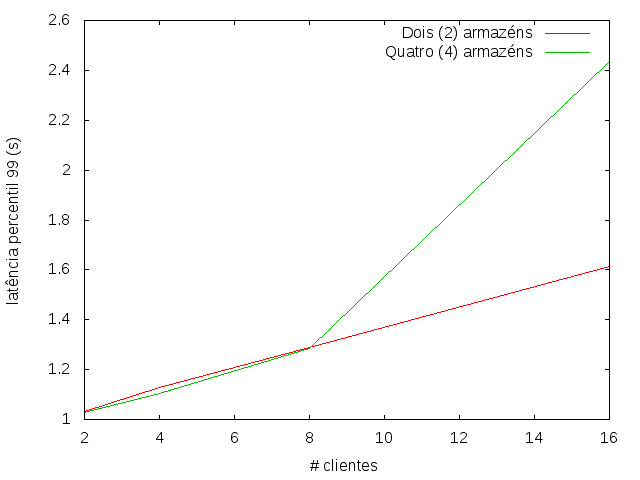
\includegraphics[scale=.4]{img/questao-1/rep-read-lat-pct99}
\caption{Percentil 99 da latência obtida de acordo com o número de clientes para dois e quatro armazéns}
\end{figure}

\newpage

\subsection{\textit{Read Uncommitted} como Método de Isolamento}

São apresentados em seguida, sobre a forma de uma tabela, os resultados obtidos na execução do \textit{benchmark} usando como Método de Isolamento o \textit{Read Uncommitted}.

\begin{table}[!h]
\center
\small
\begin{tabular}{|c|c|c|c|c|}
\hline
\textbf{\# clientes} & \textbf{\# pedidos} & \textbf{pedidos/s} & \textbf{lat. média (s)} & \textbf{lat. perct. 99 (s)}  \\ \hline
2 & 17797 & 296.6167 & 1.0090 & 1.0291  \\ \hline
4 & 20594 & 343.2303 & 1.0171 & 1.1176  \\ \hline
8 & 20852 & 347.5300 & 1.0278 & 1.2382  \\ \hline
16 & 17933 & 298.8668 & 1.0770 & 1.4699  \\ \hline
\end{tabular}
\caption{Resultados obtidos para dois (2) armazéns}
\end{table}

\begin{table}[!h]
\center
\small
\begin{tabular}{|c|c|c|c|c|}
\hline
\textbf{\# clientes} & \textbf{\# pedidos} & \textbf{pedidos/s} & \textbf{lat. média (s)} & \textbf{lat. perct. 99 (s)}  \\ \hline
2 & 17253 & 287.5477 & 1.0080 & 1.0308  \\ \hline
4 & 18406 & 306.7542 & 1.0194 & 1.1353  \\ \hline
8 & 16434 & 273.8942 & 1.0306 & 1.2895  \\ \hline
16 & 18418 & 306.9657 & 1.0667 & 1.5075  \\ \hline
\end{tabular}
\caption{Resultados obtidos para quatro (4) armazéns}
\end{table}

\newpage

A partir dos dados exibidos nas tabelas anteriores, foram desenhados os seguintes gráficos representativos do \textbf{débito} (número de pedidos por segundo), da \textbf{latência média} e do valor do \textbf{percentil 99 da latência}, interpretada, aqui, como latência máxima.

\begin{figure}[!h]
\centering
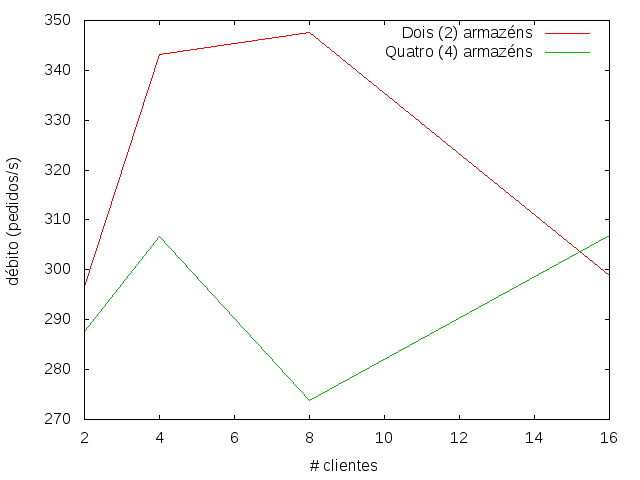
\includegraphics[scale=.4]{img/questao-1/read-uncom-deb}
\caption{Débito obtido de acordo com o número de clientes para dois e quatro armazéns}
\end{figure}

\begin{figure}[!h]
\centering
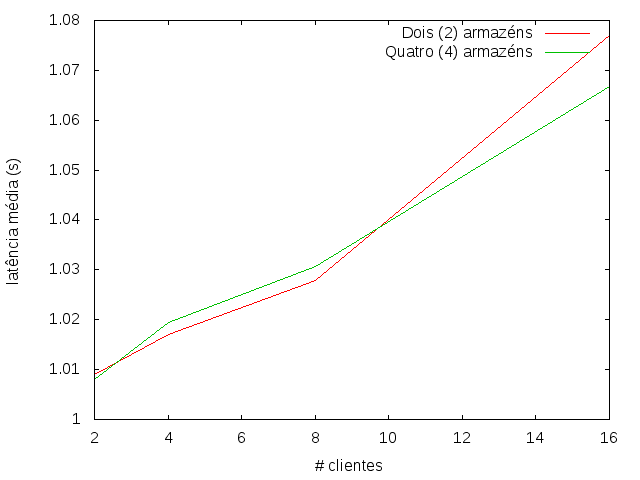
\includegraphics[scale=.4]{img/questao-1/read-uncom-lat-med}
\caption{Latência média obtida de acordo com o número de clientes para dois e quatro armazéns}
\end{figure}

%\newpage

\begin{figure}[!h]
\centering
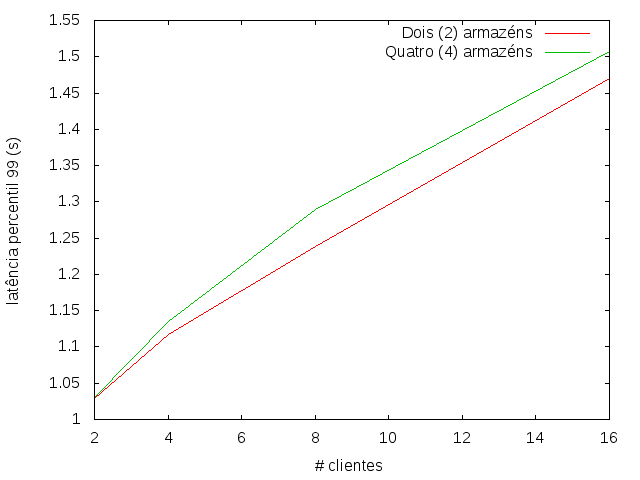
\includegraphics[scale=.4]{img/questao-1/read-uncom-lat-pct99}
\caption{Percentil 99 da latência obtida de acordo com o número de clientes para dois e quatro armazéns}
\end{figure}

\newpage
\subsection{\textit{Read Committed} como Método de Isolamento}

São apresentados em seguida, sobre a forma de uma tabela, os resultados obtidos na execução do \textit{benchmark} usando como Método de Isolamento o \textit{Read Comitted}.

\begin{table}[!h]
\center
\small
\begin{tabular}{|c|c|c|c|c|}
\hline
\textbf{\# clientes} & \textbf{\# pedidos} & \textbf{pedidos/s} & \textbf{lat. média (s)} & \textbf{lat. perct. 99 (s)}  \\ \hline
2 & 14810 & 246.8311 & 1.0114 & 1.0446  \\ \hline
4 & 20792 & 346.5310 & 1.0170 & 1.1070  \\ \hline
8 & 21509 & 358.4819 & 1.0310 & 1.2144  \\ \hline
16 & 12534 & 208.8956 & 1.0901 & 1.9881  \\ \hline
\end{tabular}
\caption{Resultados obtidos para dois (2) armazéns}
\end{table}

\begin{table}[!h]
\center
\small
\begin{tabular}{|c|c|c|c|c|}
\hline
\textbf{\# clientes} & \textbf{\# pedidos} & \textbf{pedidos/s} & \textbf{lat. média (s)} & \textbf{lat. perct. 99 (s)}  \\ \hline
2 & 17495 & 291.5808 & 1.0051 & 1.0264  \\ \hline
4 & 19219 & 320.3136 & 1.0165 & 1.1110  \\ \hline
8 & 18722 & 312.0306 & 1.0276 & 1.2623  \\ \hline
16 & 18302 & 305.0299 & 1.0609 & 1.5071  \\ \hline
\end{tabular}
\caption{Resultados obtidos para quatro (4) armazéns}
\end{table}

\newpage

A partir dos dados exibidos nas tabelas anteriores, foram desenhados os seguintes gráficos representativos do \textbf{débito} (número de pedidos por segundo), da \textbf{latência média} e do valor do \textbf{percentil 99 da latência}, interpretada, aqui, como latência máxima.

\begin{figure}[!h]
\centering
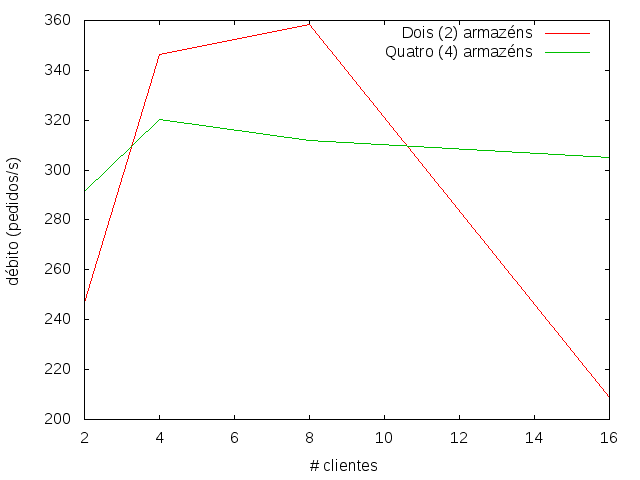
\includegraphics[scale=.4]{img/questao-1/read-com-deb}
\caption{Débito obtido de acordo com o número de clientes para dois e quatro armazéns}
\end{figure}

\begin{figure}[!h]
\centering
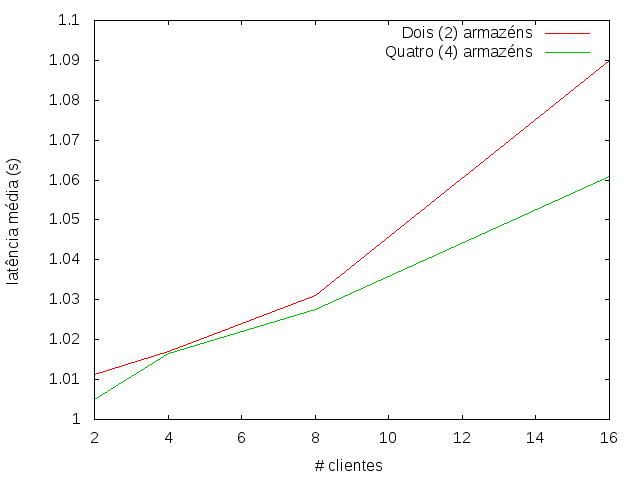
\includegraphics[scale=.4]{img/questao-1/read-com-lat-med}
\caption{Latência média obtida de acordo com o número de clientes para dois e quatro armazéns}
\end{figure}

%\newpage

\begin{figure}[!h]
\centering
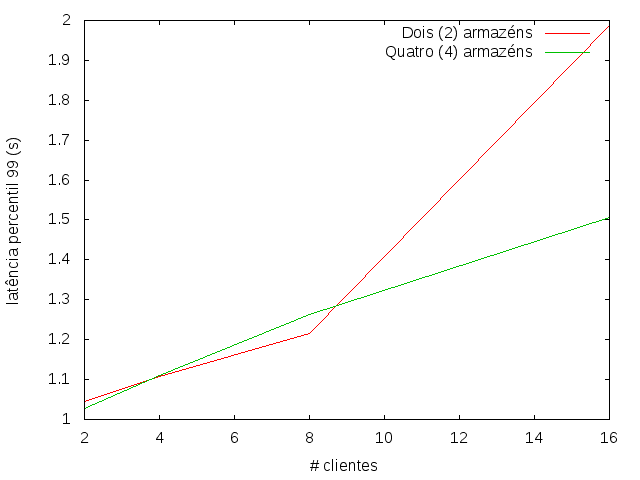
\includegraphics[scale=.4]{img/questao-1/read-com-lat-pct99}
\caption{Percentil 99 da latência obtida de acordo com o número de clientes para dois e quatro armazéns}
\end{figure}

\newpage
\subsection{Comparação dos Métodos de Isolamento e  Conclusões Finais}
